\chapter{Конструкторский раздел}\label{sec:design}

\section{Схемы алгоритмов}\label{sec:design-flowcharts}

Обращение к элементам массивов на схеме алгоритмов обозначено подстрочными индексами.
Операция присваивания обозначена как "$\leftarrow$", операции "равно" и "не равно" как "$=$" и "$\#$" соответственно.
На рисунке \ref{fig:lee-conc-parall} представлены схемы параллельного и синхронного выполнения алгоритма Ли.
На рисунке \ref{fig:lee-BFS} представлена схема поиска в ширину.
На рисунке \ref{fig:lee-wave} представлена схема распространения волны.
\begin{center}
	\begin{figure}[H]
		\centering
		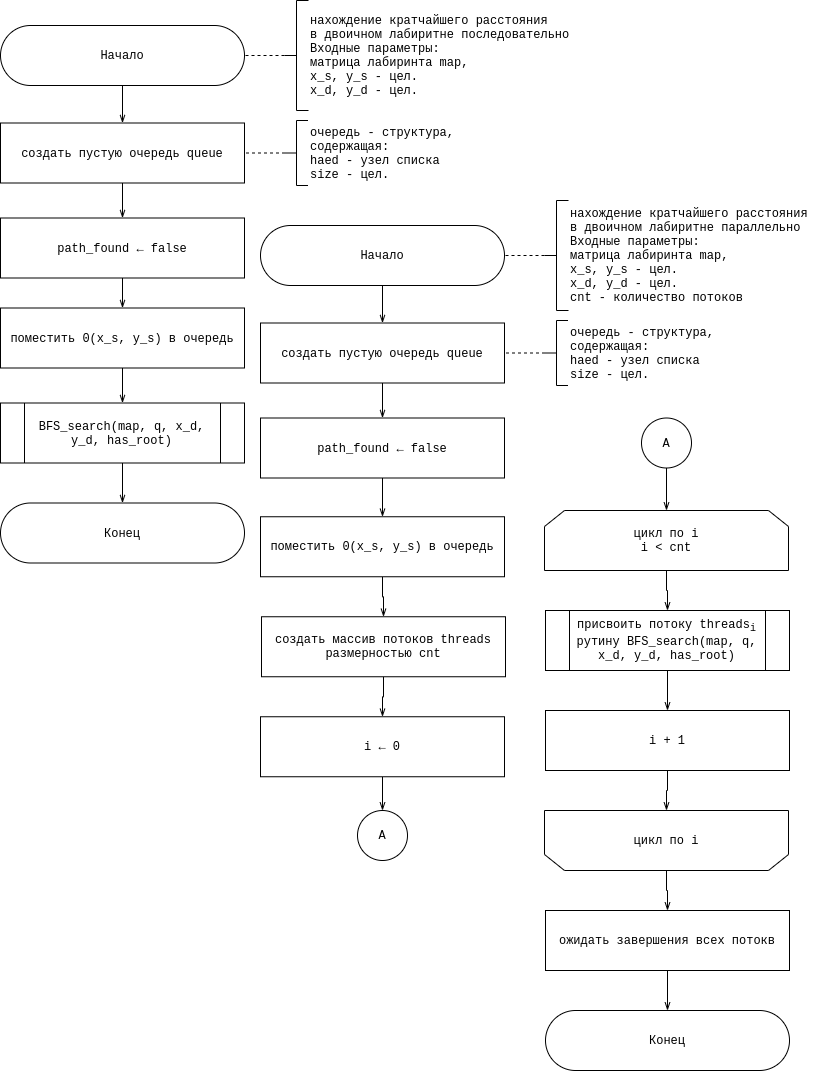
\includegraphics[width=0.9\linewidth]{assets/lee-concur-parall.drawio.png}
		\caption{Схемы синхронного и параллельного алгоритмов Ли}
		\label{fig:lee-conc-parall}
	\end{figure}
\end{center}
	
\begin{center}
	\begin{figure}[H]
		\centering
		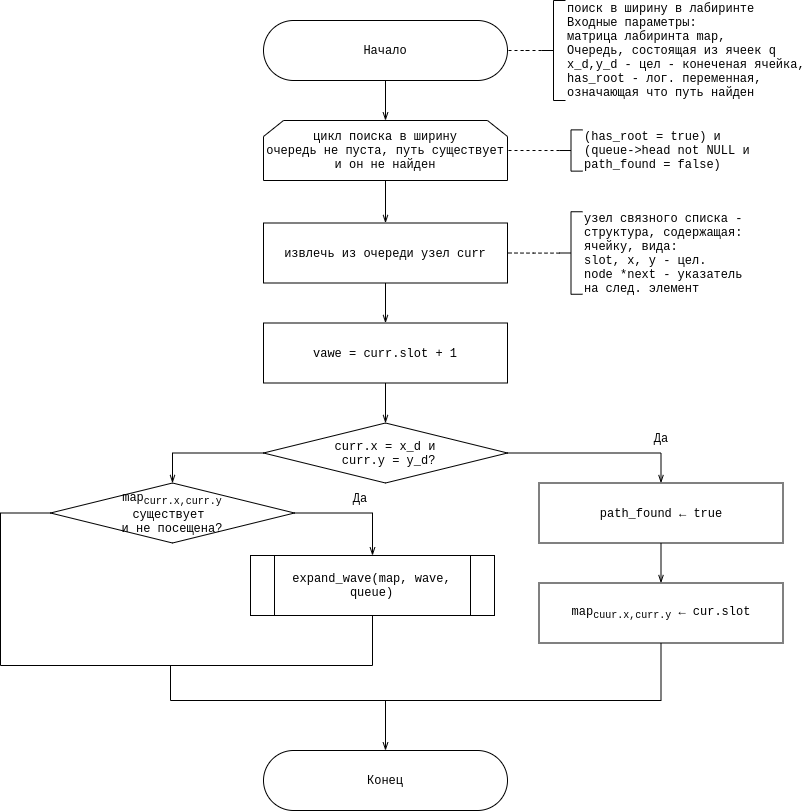
\includegraphics[width=0.9\linewidth]{assets/lee-BFS-search.drawio.png}
		\caption{Схема поиска в ширину на графе - матрице}
		\label{fig:lee-BFS}
	\end{figure}
\end{center}

\begin{figure}[H]
	\centering
	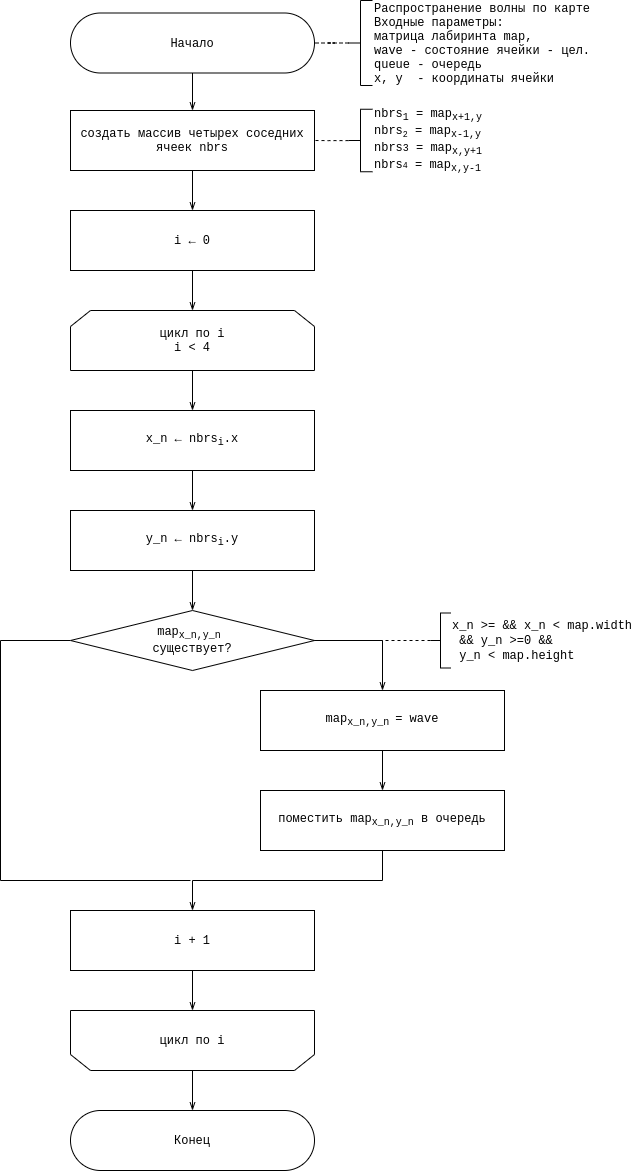
\includegraphics[width=0.75\linewidth]{assets/lee-expand-wave.drawio.png}
	\caption{Схема процедуры распространения волны}
	\label{fig:lee-wave}
\end{figure}

\subsection{Вывод}
Были разработаны схемы последовательного  параллельного алгоритма Ли. Получено достаточно теоретической информации для написания программного обеспечения, решающего поставленную задачу.
